\lstinputlisting[language=bash,basicstyle=\small]{python_codes/fieldstone_44/keywords.ascii}

\begin{center}
Code at \url{https://github.com/cedrict/fieldstone/tree/master/python_codes/fieldstone_44}
\end{center}

\par\noindent\rule{\textwidth}{0.4pt}
%%%%%%%%%%%%%%%%%%%%%%%%%%%%%%%%%%%%%%%%%%%%%%%%%%%%%%%%%%%%%%%%%%%%%%%%%%%%%%%%%%%%%%%%%%%%

WORK in PROGRESS. I am stuck because:

I need a list of nodes on the boundary
I need a GCOORD.txt file with more decimals, bc of boundary conditions issues.
I need an even lower resolution  grid
I need the scaling factors for rho,eta, ...


\begin{center}
\includegraphics[width=7cm]{python_codes/fieldstone_44/grid_lowres2}
\includegraphics[width=7cm]{python_codes/fieldstone_44/grid_lowres3}\\
\includegraphics[width=7cm]{python_codes/fieldstone_44/grid_lowres4}
\includegraphics[width=7cm]{python_codes/fieldstone_44/grid_lowres5}
\end{center}

371km, 300km depth, 660km depth, 1500km.

\begin{center}
\includegraphics[width=14cm]{python_codes/fieldstone_44/sifg19}\\
{\captionfont Taken from \cite{sifg19}}
\end{center}


\begin{center}
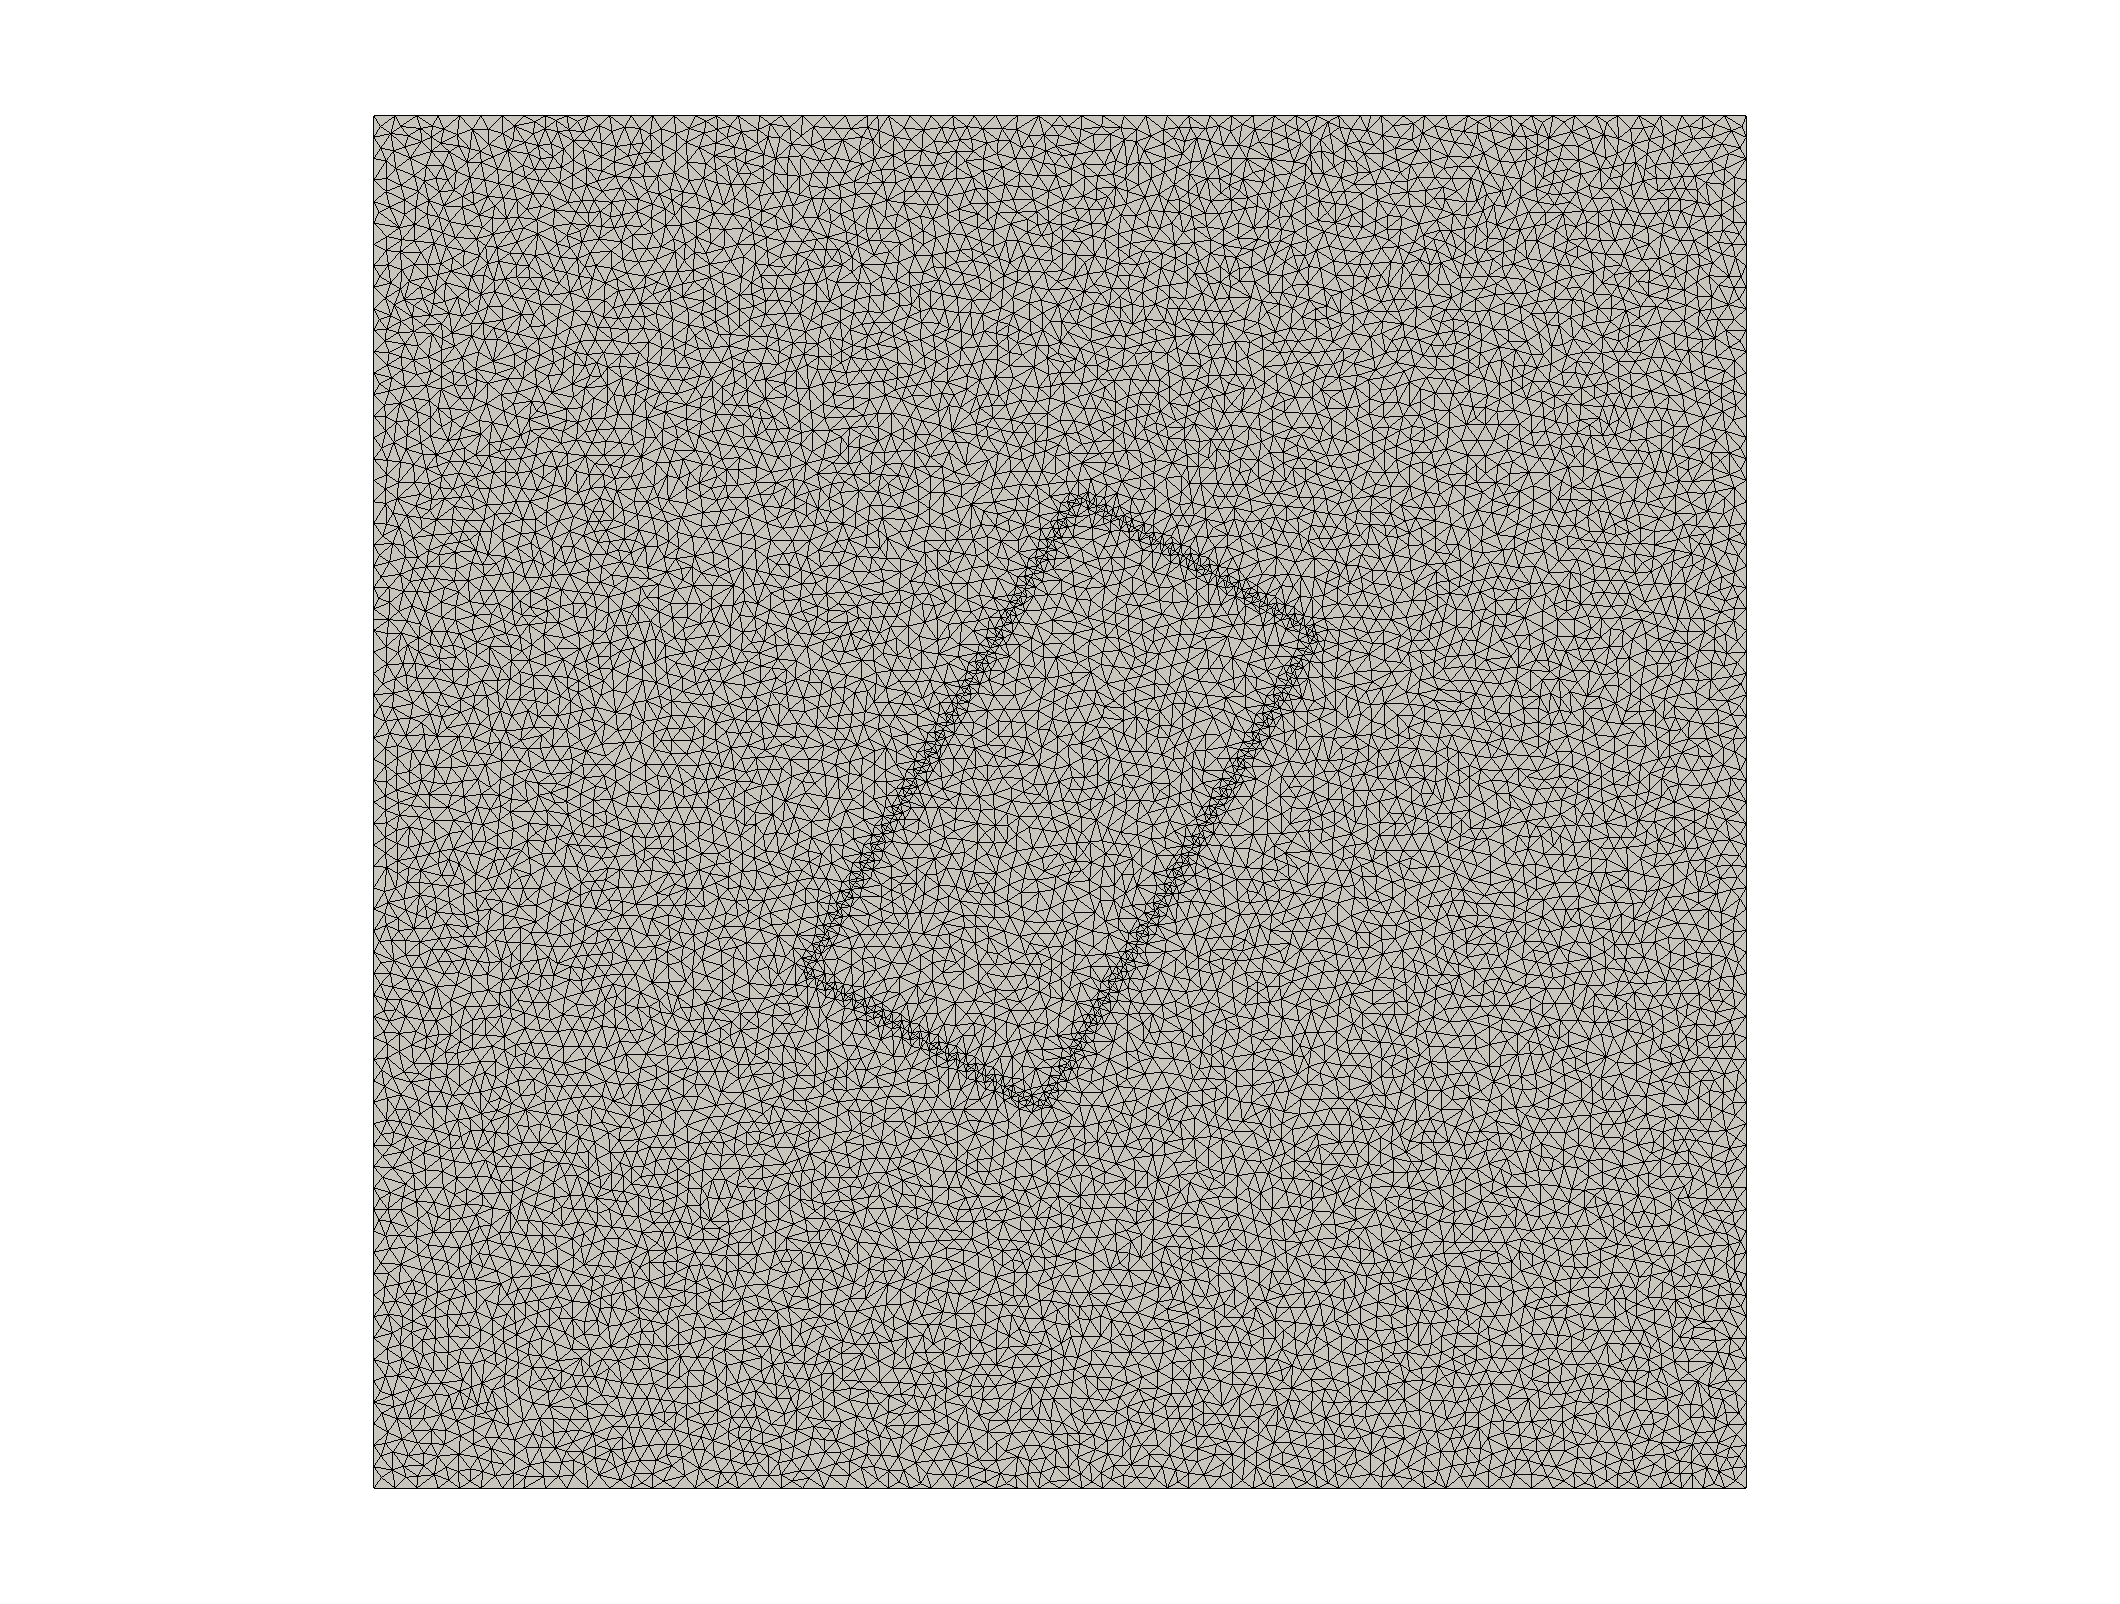
\includegraphics[width=7cm]{python_codes/fieldstone_44/results/mesh}
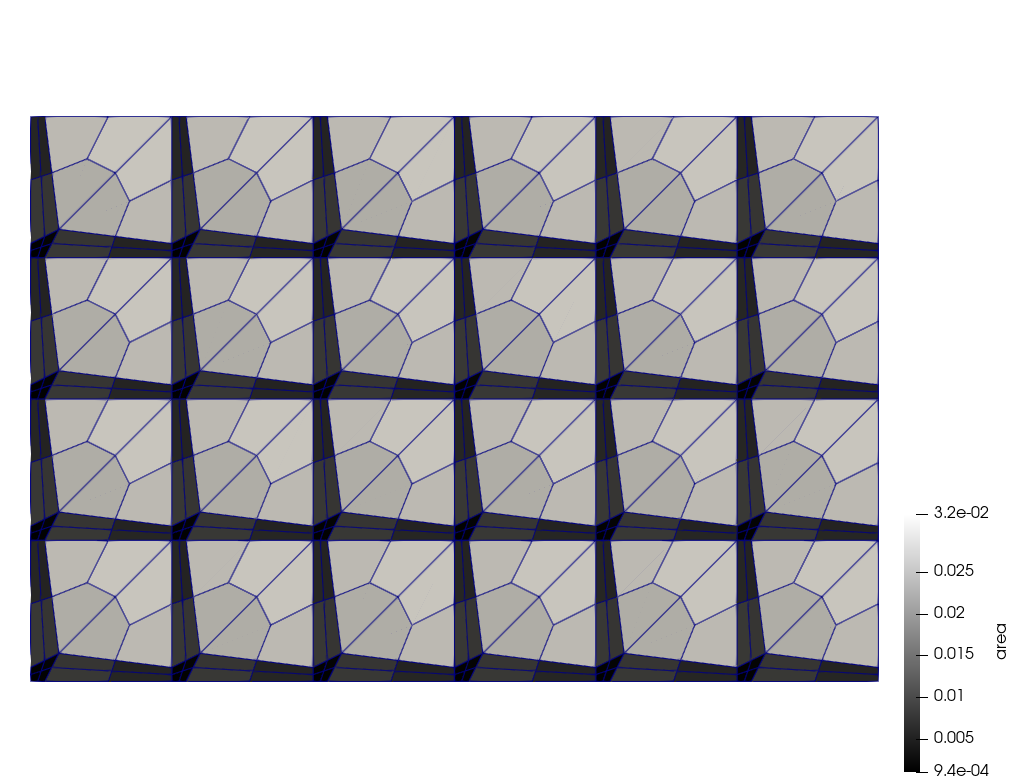
\includegraphics[width=7cm]{python_codes/fieldstone_44/results/area}\\
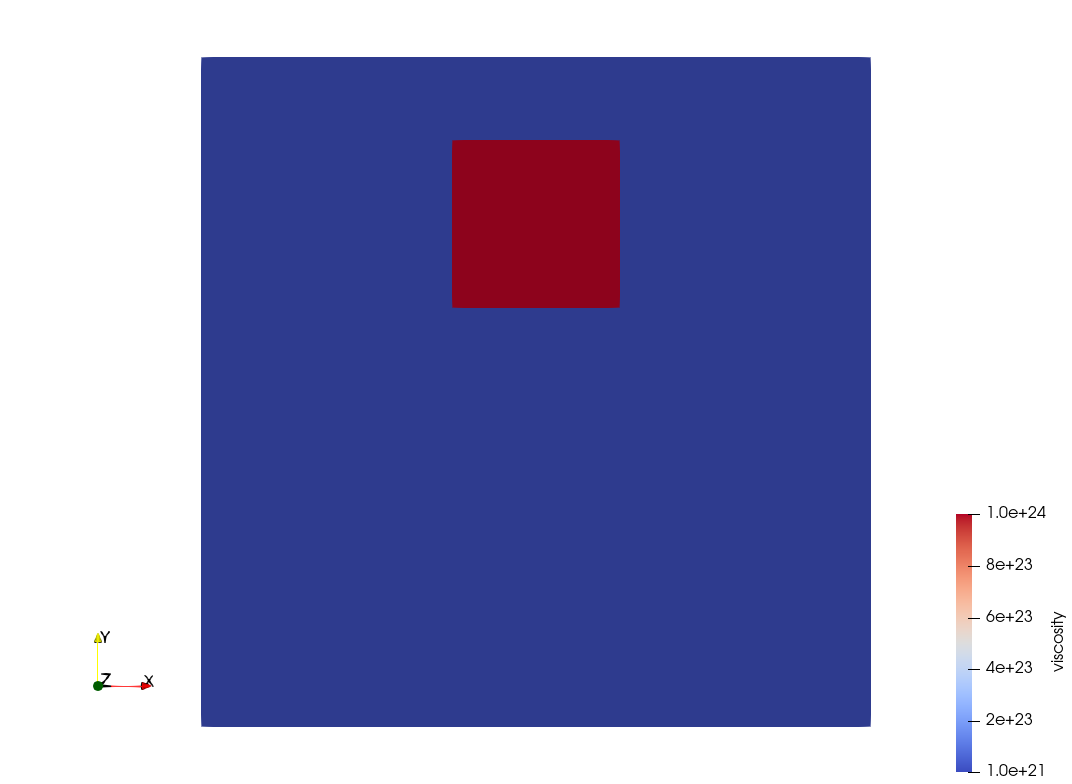
\includegraphics[width=7cm]{python_codes/fieldstone_44/results/eta}
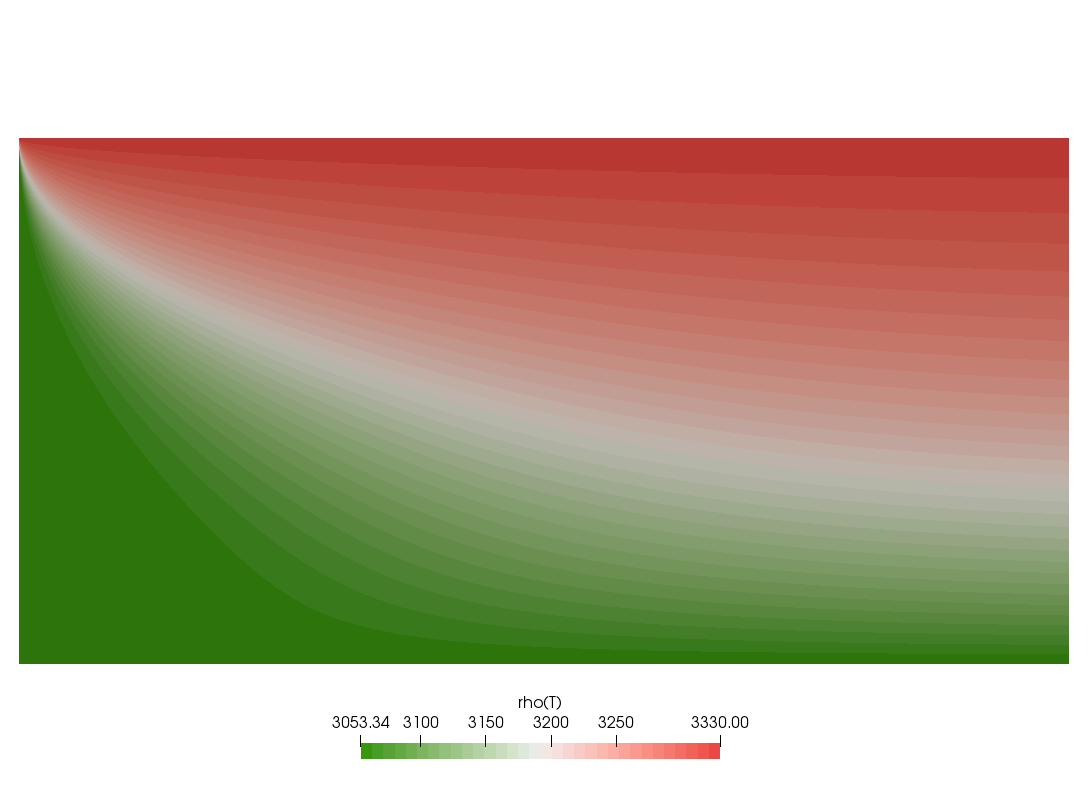
\includegraphics[width=7cm]{python_codes/fieldstone_44/results/rho}\\
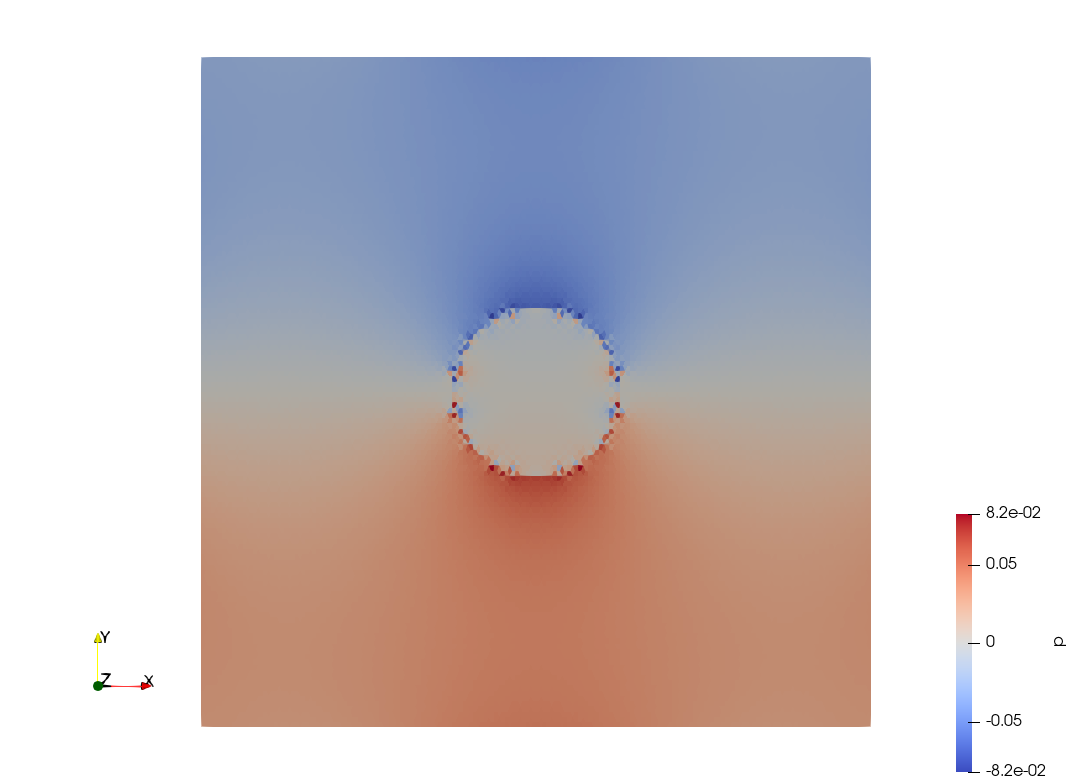
\includegraphics[width=7cm]{python_codes/fieldstone_44/results/p}
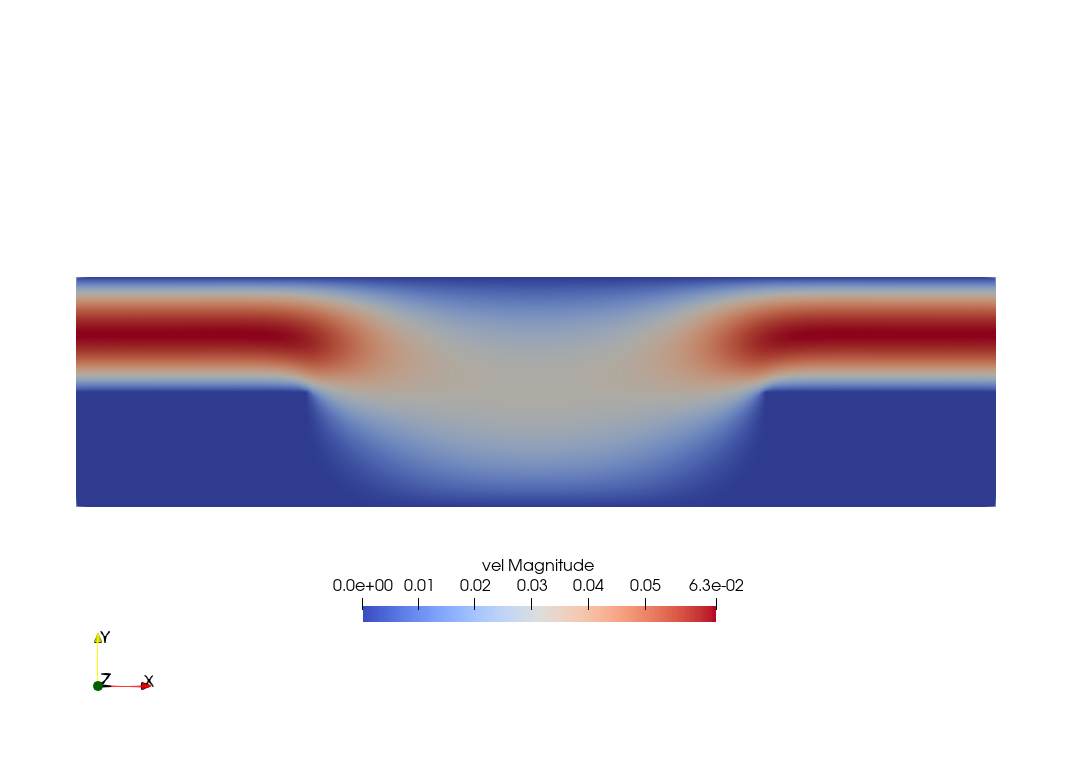
\includegraphics[width=7cm]{python_codes/fieldstone_44/results/vel}
\end{center}
